\documentclass{article}
\usepackage[utf8]{inputenc}
\usepackage{listings}
\usepackage{color} 
\usepackage{hyperref}
\usepackage{float}
\usepackage{subcaption}
\usepackage{asmath}


\hypersetup{
    colorlinks=true, %set true if you want colored links
    linktoc=all,     %set to all if you want both sections and subsections linked
    linkcolor=blue,  %choose some color if you want links to stand out
}

%\usepackage{titling}
\usepackage{graphicx}
%\usepackage{titlepic}

\lstset{
	frame=tb, % draw a frame at the top and bottom of the code block
   	tabsize=4, % tab space width
   	showstringspaces=false, % don't mark spaces in strings
    numbers=left, % display line numbers on the left
    commentstyle=\color{red}, % comment color
    keywordstyle=\color{blue}, % keyword color
    stringstyle=\color{green} % string color
}


\title{\vspace*{\fill} \textbf{COP 290 Assignment 3}
	  \\ {\Large \textbf{Ping Pong Game}}
	  % \\  \vspace{3mm} \includegraphics{ddlogo.png}}
}
\author{
	\vspace{5mm} \\
	 \textbf{Aditi}\\
	2014CS10205 \vspace{2mm} \\
	\textbf{Ayush Bhardwaj}\\ 
	2014CS10091 \vspace{2mm} \\
	\textbf{Nikhil Gupta}\\ 
	2014CS50462 \vspace{2mm}
}
\date{\vspace{3mm} \textbf{April 2016} \vspace*{\fill}}

\begin{document}
	\maketitle

	\newpage

	\tableofcontents

	\newpage

	\section{Objectives}
	Design a desktop app which is:
	\begin{itemize}
	\item Simulation of Multi player and Multilevel Ping Pong game.
	\item Allows multiple players to play at one time using p2p networking.
	\item Every client controls its own game state on the basis of information transfer.
	\end{itemize}

	\section{Overall Design}
		The game involves each player having a rectangular paddle, using which he has to prevent the balls from colliding with the walls of the walls. Each time the paddle misses a ball, the player loses one life. The player has a limited number of lives and has to score the maximum in them.The game would be controlled via a runnable function which is called again and again till the game ends.All the events of the game would be handled by this function. According to the requirements of the assignment:
				\begin{itemize}
			\item Each peer back-end will be programmed in Java using sockets.
			\item Doxygen will be used to create HTML documentation of the entire code base.
			\item The entire code will be split up in multiple files to ensure modularity in code.
			\item Swing library will be used to display the Graphic User Interface.
		\end{itemize}
	\section{Graphical User Interface}
	
    	\subsection{Start Screen}
    	The Start Screen will handle the setting up of the game. It will offer options like Play Against Computer, Play with peers, Number of Players,No of balls,Level of Difficulty. After this screen, another screen to establish connection with other players will appear.

    	\subsection{Main UI}
    	The main user interface displays the board as a JFrame object along with the balls and the paddles at any instant of time. Balls will be modeled as 2-dimensional circles.
    	\par\noindent The \textbf{Swing library} ~\cite{swing_java} of Java language will be used to render the interface. At every instant of time, data from the object of class Board will be extracted, to get information about all the balls and the paddles to be displayed on screen. The colors for the balls are randomly chosen, but the radius for all of them is constant for one particular game.Some of the features of UI are:
    	\begin{itemize}
    	\item Rectangular Board will have \textbf{triangular corners}. Balls will be moving on it continuously. Paddles will move according to the player's moves.
    	\item Every user will see his own paddle on the bottom edge of the board.
    	\item Number of Lives remaining will be displayed for each player in the form of hearts.
    	\item \textbf{Power Ups(or Downs)} will be random floating objects on the board. They will be randomly generated and will move in random directions.
    	\item There will be suitable functions to render the change in paddle on collection of a Power Up or Down.
    	\item The user controls his paddle position by using the \textbf{keyboard} Left/Right keys or by using the \textbf{Left/Right buttons} on screen or by dragging the paddle on the window using the \textbf{Mouse pointer}.
    	\end{itemize}

	    \begin{figure}[H]
      \centering
      \begin{subfigure}{.4\textwidth}
          \centering
          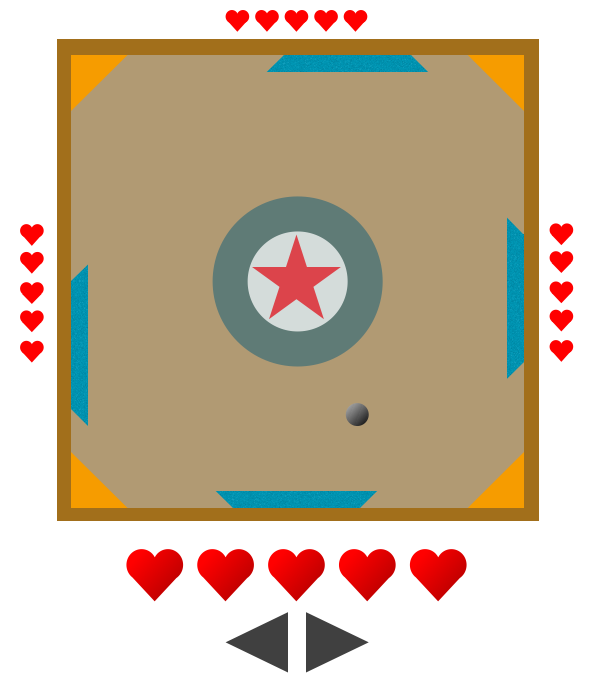
\includegraphics[width=0.9\linewidth]{UI.png}
          \caption{Splash Screen}
          \label{fig:sub1}
      \end{subfigure}
    \end{figure}


	\section{Sub Components}
	The following classes would be needed to design an efficient back end.
\subsection{Design Of The Ball} Ball class consist of all the information about the balls on board i.e. its velocity, position, radius and color.
\lstset{
    frame=tb, % draw a frame at the top and bottom of the code block
    tabsize=4, % tab space width
    showstringspaces=false, % don't mark spaces in strings
    numbers=left, % display line numbers on the left
    commentstyle=\color{red}, % comment color
    keywordstyle=\color{blue}, % keyword color
    stringstyle=\color{green} % string color
}


\begin{lstlisting}[language=Java, caption={Class Parameters for Ball}]
class Ball
{
	private:
		double radius;              //Radius of the ball
		double center_x;            //X coordinate of the center of ball
		double center_y;            //Y coordinate of the center of ball
		double velocity_x;          //X component of the velocity of ball
		double velocity_y;          //Y component of the velocity of ball
		ArrayList<float> color;   	//Color in RGB format of ball
};

\end{lstlisting}

Functions will be made for accessing all the data parameters of the ball and updating them as desired. Functions for obtaining a random ball based on the desired range will also be created.

\subsection{Design of Paddles} The Paddle class would contain all the information regarding one paddle. Basic functions will be there to retrieve all the data related to one paddle. All paddles would have the same color.

\begin{lstlisting}[language=Java, caption={Class Parameters for Paddle}]
class Paddle
{
	private:
		double length;              //Length of paddle
		ArrayList<float> color;   	//Color in RGB format of paddle
		double paddle_x;			// x coordinate of paddle center
		double paddle_y;			// y coordinate of paddle center
		int times_ball_missed;		// no of times this paddle has missed ball
		bool isAlive;				// denotes if player is still alive
};

\end{lstlisting}

\subsection{Design Of The Board} The background screen would be implemented using a Board class. It would consist of all the information about the background i.e. its dimensions, color, number of balls present and a vector containing the information of the balls and similarly for all the alive paddles.

\begin{lstlisting}[language=Java, caption={Class Parameters for Board}]
class Board
{
	private:
		float dimension_x;                   //x dimension of board
		float dimension_y;                   //y dimension of board
		int number_balls;                    //number of balls on board
		ArrayList<Ball> vector_of_balls;     //vector of balls on board
		int number_paddles;					 // number of paddles, i.e. players
		ArrayList<Paddle> vector_of_paddles; // vector of paddles on board
		ArrayList<bool> dead_alive;	// array for whether player is alive/dead
};

\end{lstlisting}

Functions for accessing and updating the parameters of the board will be created. Apart from this, functions to add or remove particular balls will be provided.

			\section{Physics} 
			\par\noindent The basic law of physics will hold throughout the game.We will be handling the following events:
			\begin{itemize}
			\item \textbf{Motion of the Ball:} Instantaneous velocities of the ball would be maintained in X and Y directions.Next positions would be calculated simply by adding these to the current X and Y positions. 
			\item \textbf{Motion of the Paddle:} Movement of paddle can be controlled via Mouse or the Keyboard. In case of Mouse, current position of the mouse will control the movement of paddle. While in case of Keyboard, Arrow Keys will control the paddle movements.
			\item \textbf{Collision of Ball and Paddle:} Collision occurs whenever the distance between the center of ball and paddle boundary is less than the ball's radius.Basic collision equation will be used while also considering the speed of the paddle at the time of collision. A suitable coefficient of restitution would be used.
			\item \textbf{Collision of Ball and Boundary:} The detection of this collision is also similar to the one listed above. Basic collision equation will be used. A suitable coefficient of restitution would be used.
			\item \textbf{Collision between balls:} Basic equations for head on collision between two solid objects would be used to calculate the next velocities of both the balls.
			\item \textbf{Corner Case:} As design of all boundaries(of paddles, board) are of triangular shape, Corner Cases reduce to a simple collision between the ball and straight boundaries. The boundary with which the client first detects the collision is considered for the calculation.
			\item \textbf{Our Equations}
			\begin{enumerate}
				\item   \[V_{y2} = U_{x1}(\frac{\epsilon + 1}{2})cos\theta sin\theta + U_{y1}(\frac{\epsilon + 1}{2})sin^2\theta + U_{x2}((\frac{1 - \epsilon}{2})cos\theta sin\theta - sin\theta cos\theta) + \\ U_{y2}((\frac{1 - \epsilon}{2})sin^2\theta + cos^2\theta) \] 

				\item \[V_{x2} = U_{x1}(\frac{\epsilon + 1}{2})cos^2\theta + U_{y1}(\frac{\epsilon + 1}{2})sin\theta cos\theta + U_{x2}((\frac{1 - \epsilon}{2})cos^2\theta + sin^2\theta) + \\ U_{y2}((\frac{1 - \epsilon}{2})sin\theta cos\theta - cos\theta sin\theta) \]
				\item \[ V_{y1} = U_{x1}((\frac{1 - \epsilon}{2})cos\theta sin\theta - cos\theta sin\theta) + U_{y1}((\frac{1 - \epsilon}{2})sin^2\theta + cos^2\theta) + U_{x2}(\frac{\epsilon + 1}{2})cos\theta sin\theta + // U_{y2}(\frac{1 - \epsilon}{2})sin^2\theta \]
				\item \[ V_{x1} = U_{x1}((\frac{1 - \epsilon}{2})cos^2\theta - sin^2\theta) + U_{y1}((\frac{1 - \epsilon}{2})cos\theta sin\theta - cos\theta sin\theta) + U_{x2}(\frac{\epsilon + 1}{2})cos^2\theta + \\ U_{y2}(\frac{1 - \epsilon}{2})sin\theta cos\theta \]

				\end{enumerate}

			\end{itemize}
			

			\section{Computer Player Algorithm}
			\par\noindent The computer player can have variable speed. But the range of speed varies on the basis of level of difficulty.Algorithm used by computer would be based on the following facts:

			\begin{itemize}
			\item Initially computer player tries to align its paddle center with the center of the closest ball moving towards it.
			\item When the ball is about to reach a wall, the computer player first calculates according to the assumption of a static paddle and moves.
			\item After the collision has occurred, the computer again moves accordingly.
			\item Another event will be choosing between ball catching versus catching power up objects. The decision will basically be based upon the distance of the power up object and the expected distance of the ball from the paddle after collision.
			\end{itemize}

			\section{p2p Networking}
			\par\noindent We would use socket programming ~\cite{socket_java} to implement p2p networking model. Each client has (n - 1) sockets, one for interaction with all the other n-1 players. Each client sends the following information to its peers:
			\begin{itemize}
			\item \textbf{Loss of Life:} Boolean value denoting whether the player has missed the ball and lost a life..
			\item \textbf{Current data of paddle:} Position of paddle is sent,  other clients adjust the position of the paddle on their board accordingly. 
			\item \textbf{Collision with paddle:} Boolean value denoting collision along with the new position and velocity of ball would be sent.
			\item \textbf{Collection of PowerUps} An integer mapped to a specific power up would be sent.Client will render the UI accordingly.
			% ADD MORE, AYUSH TODO
			\end{itemize}
			\subsection{Event Flow}
			The steps involved in flow of each network message from Peer 1 to Peer 2 are:
			\begin{enumerate}
			\item Peer 1 initiates the process of sending the message
			\item Peer 1 tries to establish the connection with the peer
			\item Peer 2 accepts the connection and starts the handler thread
			\item Peer 1 sends the message
			\item Peer 2 receives the message and send backs the acknowledgment back to peer 1 and closes the connection.
			\end{enumerate}
			The flow is similar for any Sender and Receiver pair.
			\subsection{Event Handling}
			\begin{enumerate}
			\item \textbf{Missing the ball:} Player looses a life if the ball misses the paddle and touches the wall.It involves updating of the number of remaining lives of the player.
			\item \textbf{Disconnection: }If a peer takes more than an specified time to answer, it is disconnected. In case a particular client is disconnected from the network, a pop up would be displayed to the other players, and according to their decision, a computer player will be added or the game would continue with the player removed.
			\item \textbf{Updating Position: }Every client adjusts the paddle positions of other client, according to the data received. Next position of the ball is calculated individually by the clients or is updated in case of collision with any other peer. All the data is consistent throughout the game for all the players.
			\item \textbf{Collection of Power Up:}Communicated via the network message and a suitable method is called to update the UI.
			\end{enumerate}
			

	\section{Thread Interactions}
	\par\noindent We would need multiple threads ~\cite{thread_java} to handle different components of the game separately. There would be separate runnable() functions for the following list of threads to be used:
	\begin{itemize}
	\item \textbf{Update UI} : This thread continuously updates the positions of the balls and the paddles being displayed to the user, on the basis of the information received from the network. This is done after every fixed interval of time.
	\item \textbf{One Thread Per Socket} : There would be n-1 threads, each controlling communication with one of the other clients. Each thread is responsible for making the connection via sockets using unique ports and sending and receiving information about the states of the paddles over network.
	\end{itemize}
	\par\noindent The thread maintaining UI will call the update() function only after receiving the updated information from the other n-1 threads.

	\section{Testing Of Components}
		% \begin{enumerate}
			\subsection{Single peer testing}
				\begin{itemize}
					\item Unit testing will be used to check if the socket connections are transferring information correctly.
					\item For each peer to peer socket, stress testing will be done via python or bash scripts to verify that the socket connections perform as expected in various situations.
				\end{itemize}

			\subsection{Computer Player Testing}
			We will play against the computer algorithm both on single PC as well as in a network of less than four players.
			\subsection{Overall p2p Testing}
				We will use the app on our desktops once it is ready to identify and squash any remaining bugs.
	\section{Extra Features}
	\begin{itemize}
	\item Every player gets an option of choosing the orientation of the board visible to him, according to his comfort.
	\item Special items would be floating around on the board, which on being captured, will provide the player with special powers.
	\item The special powers include : extra speed of paddle, more length of paddle, slower ball close to the player's paddle and extra points.
	\item Some danger items would also be floating, which on being captured, would either slow down the paddle, or reduce its length or make the ball faster in the player's region.
	\item The game would have multiple levels that would differ by increasing ball speed and decreasing paddle length.
	\item While considering collision, frictional drag will also be considered.
	\item Corners of the board and the paddles will be triangular.
	\item Players can play with more than one balls also.
	\end{itemize}

	\section{Future Endeavors}
	\begin{itemize}
	\item The 2D game can be translated into 3D using a 3D rendering software to give an in-depth gaming experience. 
	\end{itemize}

	\section{Source Code}
	The source code of the project is maintained in the following repository: \\
	\url{https://github.com/aditi741997/COP290_PingPong.git}
	\bibliographystyle{abbrv}
	\medskip
	\bibliography{references}
	% TODO: Add some links here
\end{document} 
